\iffalse
%\documentclass{article}
\usepackage[dvipsnames]{xcolor}
\usepackage{tikz}
\usetikzlibrary{positioning,calc,backgrounds,fit,arrows.meta}
\usetikzlibrary{arrows}
\usetikzlibrary{decorations.pathreplacing,calligraphy}


\fi
%\begin{document}
\newcommand{\lastidx}{n+1}
\newcommand{\evalidx}{n+1}
\newcommand{\setofpairs}[2]{\{(x_1^{#1}, y_1^{#1}),\dots,(x_{#2}^{#1}, y_{#2}^{#1})\}}
\newcommand{\seq}[1]{$\setofpairs{#1}{\lastidx{}}$}
\newcommand{\xypair}[1]{$(x_{#1},y_{#1})$}
\newcommand{\qattbend}{40}
\def\innerdistance{2.2em}
\def\outdistane{1.2em}
\def\indistane{1.em}
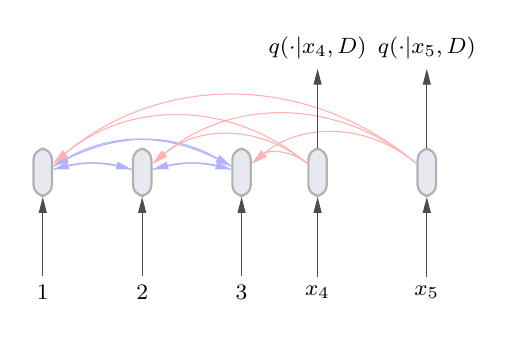
\begin{tikzpicture}[remember picture,
  inner/.style={circle,draw=blue!50,fill=blue!20,thick,inner sep=3pt},
]
\tikzstyle{bigbox} = [thick, fill=white, rounded corners, rectangle,draw=black!30]
\tikzstyle{sample} = [thick, minimum size=0.6cm, rounded corners,rectangle, fill=Salmon!10,draw=black!30]
\tikzstyle{loss} = [thick, minimum size=0.6cm, rounded corners,rectangle, fill=PineGreen!10,draw=black!30]
\tikzstyle{timestep} = [thick,minimum width=0.2cm,minimum height=.6cm, rounded corners,rectangle, fill=MidnightBlue!10,draw=black!30]
\tikzstyle{querytimestep} = [thick,minimum width=0.2cm,minimum height=.6cm, rounded corners,rectangle, fill=MidnightBlue!10,draw=black!30]
\tikzstyle{innerattention} = [draw=blue!30,-{Triangle[length=2mm, width=1mm]},]
\tikzstyle{queryattention} = [draw=red!30,-{Triangle[length=2mm, width=1mm]},]
\tikzstyle{output} = [draw=black!70,-{Triangle[length=2mm, width=1mm]},]
\tikzstyle{input} = [draw=black!70,-{Triangle[length=2mm, width=1mm]},]
\tikzstyle{every node} = [font=\footnotesize,]




\node[timestep] (t1) {};
\node[timestep, right=\innerdistance of t1] (t2) {};
\node[timestep, right=\innerdistance of t2] (t3) {};


\draw [ innerattention] (t1) to [bend left=15] (t2);
\draw [ innerattention] (t1) to [bend left=30] (t3);
\draw [ innerattention] (t2) to [bend right=15] (t1);
\draw [ innerattention] (t2) to [bend left=15] (t3);
\draw [ innerattention] (t3) to [bend right=30] (t1);
\draw [ innerattention] (t3) to [bend right=15] (t2);


\node[below=\indistane of t1] (i1) {\xypair{1}};
\draw [ input] (i1) -- (t1);
\node[below=\indistane of t2] (i2) {\xypair{2}};
\draw [ input] (i2) -- (t2);
\node[below=\indistane of t3] (i3) {\xypair{3}};
\draw [ input] (i3) -- (t3);

%\draw [pen colour={black!70},
%    decorate, 
%    decoration = {calligraphic brace, mirror,
%        raise=.7em,
%        amplitude=5pt}] (i1.west) --  (i3.east)
%    node[pos=0.5,below=1.2em,black]{$D$};


\node[querytimestep, right=2em of t3] (q1) {};
\node[querytimestep, right=3.2em of q1] (q2) {};


\draw [ queryattention] (q1) to [bend right=40] (t1);
\draw [ queryattention] (q1) to [bend right=40] (t2);
\draw [ queryattention] (q1) to [bend right=40] (t3);


\draw [ queryattention] (q2) to [bend right=40] (t1);
\draw [ queryattention] (q2) to [bend right=40] (t2);
\draw [ queryattention] (q2) to [bend right=40] (t3);
\node[above=\outdistane of q2] (d2) {$q(\cdot|x_5,D)$};

\node[above=\outdistane of q1] (d1) {$q(\cdot|x_4,D)$};
\draw [ output] (q1) -- (d1);
\node[] at (q1|-i1) (i4) {$x_4$};
\draw [ input] (i4) -- (q1);
\draw [ output] (q2) -- (d2);
\node[] at (q2|-i1) (i5) {$x_5$};
\draw [ input] (i5) -- (q2);
\end{tikzpicture}
%\end{document}